\documentclass{article}

\usepackage[margin=1.00in]{geometry}

\usepackage{listings}
\usepackage{diagbox}
\usepackage{mathtools}
\usepackage{rotating}
\usepackage{makecell}
\usepackage{amssymb}
\usepackage{amsmath}
\usepackage{graphicx}
\usepackage{csquotes}
\usepackage[title]{appendix}
\graphicspath{{figures/}} % Directory in which figures are stored
\usepackage{color}
\usepackage{array}
\usepackage{hyperref}
\hypersetup{
    colorlinks=true,
    linkcolor=blue,
    filecolor=blue,      
    urlcolor=blue,
    citecolor=black
}

\usepackage{longtable}
\usepackage{ulem}
\usepackage{enumitem}
\usepackage{relsize}
\usepackage{movie15}
\usepackage{natbib}
\usepackage{gensymb}

\begin{document}


\LARGE\textbf{Compaction Model Documentation}
\normalsize

\today
\author{Matt Lees}

\abstract Currently preliminary, keeping track of what my compaction model does.

%\begin{appendix}
%	\listoffigures
%\end{appendix}

\tableofcontents

\section{Fundamental Equations and Math}

\subsection{Diffusion Equation in Clays}
\label{sec:diffusion}

In order to calculate compaction, I first need to know the changing hydraulic head within all layers. In sand layers, I measure the changing head. However in clay layers I do not, and we have to calculate the evolution of head according to the 1D groundwater flow equation. The full equation which should be solved is shown neatly in \cite{helm_one-dimensional_1975} and reproduced here in Equation \ref{eq:diffusion-eqn}.

\begin{equation}
\frac{K_v}{S_s} \frac{\partial^2h}{\partial z^2} = \frac{\partial h}{\partial t} - \frac{1}{\rho g} \frac{\partial \sigma}{\partial t}
\label{eq:diffusion-eqn}
\end{equation}
$K_v$ is the vertical hydraulic conductivity, $S_s$ is the specific storage, $ h$ is hydraulic head, $z$ is the spatial dimension, $ t$ is time, $ \rho$ is the density of water, $ g $ is the gravitational constant and $\sigma$ is the overburden stress. Note that here, overburden stress refers to stress initiating \textit{above} that layer, so is not a function of the head in the layer itself. See \cite{helm_one-dimensional_1975} for discussion of this; it can be confusing because in the compaction equations, overburden stress does change with head within the layer.

There are various elements to this equation and its solution (including initial conditions and boundary conditions) which I can have as options in my code. I summarize these in Table \ref{table:diffn-options}. Note that the options I actually code up may change over time as priorities shift.

\begin{table}[h]
\centering
\begin{tabular}{|c|c|p{4cm}|} 
\hline
\textbf{Aspect} & \textbf{Option(s)} & \textbf{Options Included?} \\ 
\hline
Overburden term & Include / ignore & Yes\\
Variability of $S_s$ & None / elastic-inelastic / continuous & Yes, first do none then elastic-inelastic then continuous \\
Interbed thicknesses & Equivalent thickness / Exact thicknesses  & No. Always do exact thicknesses.\\
Interbed solution method & Analytic / Finite Difference & No. Always finite difference.  \\
Initial Condition & Constant head / other & No. Always constant head, model must be run for long enough that IC isn't important. \\ 
\hline 
\end{tabular}
\caption{Options for solving the diffusion equation within clays.}
\label{table:diffn-options}
\end{table}


\subsubsection{Existing Codes}

MODFLOW has two packages which calculate subsidence: the Subsidence and Aquifer-System Compaction (SUB) package and the Subsidence and Aquifer-System Compaction Package for Water-Table Aquifers. My principle is to always include as much detail as these packages, if not more. In the future, I may therefore note here what options they offer/require with regards to TABLE above.

\begin{table}[h]
\centering
\begin{tabular}{|c|c|p{4cm}|} 
\hline
\textbf{Aspect} & \textbf{Option(s)} & \textbf{SUB} \\ 
\hline
Overburden term & Include / ignore & Ignore \\
Variability of $S_s$ & None / elastic-inelastic / continuous & Elastic-inelastic  \\
Interbed thicknesses & Equivalent thickness / Exact thicknesses & Equivalent thicknesses for clays with the same K and S values \\
Interbed solution method & Analytic / Finite Difference & Finite difference \\
Initial Condition & Constant head / other & Constant head \\ 
\hline 
\end{tabular}
\caption{Options the various MODFLOW sub packages include.}
\label{table:diffn-options}
\end{table}

\subsubsection{Convergence of Explicit Finite Difference Solvers}

The simplest method to solve Equation \ref{eq:diffusion-eqn} numerically will be by an explicit finite different approximation. In this case, there are requirements on the temporal and spatial discretisation, as well as the value of the diffusivity parameter, for the solution to be convergent. Although this problem does not seem to have been extensively studied in the case of heterogeneous diffusivity, I found one example giving a guide for the stability criteria. In the example, the diffusion equation is written general as in Equation \ref{eq:diffusion-eqn-general}. Then, the criteria for convergence is given in Equation \ref{eq:convergence-criterium}.

\begin{equation}
\frac{\partial u}{\partial t} = \nabla \cdot (k(x) \nabla u)
\label{eq:diffusion-eqn-general}
\end{equation}

\begin{equation}
\frac{\Delta t}{\Delta x ^2} < \frac{1}{2 max(k)}
\label{eq:convergence-criterium}
\end{equation}
where $\Delta t$ is the timestep and $\Delta x$ is the discretisation in the spatial dimension.

This criterion may seem counter intuitive at first, as it means that a larger $\Delta x$ gives better convergence for a fixed $\Delta t$. The way to think of this is as a trade-off: it is hardest to have both good spatial and temporal resolution simultaneously.

\subsubsection{Impact of allowing overburden stress to change}
\label{sec:overburden-gwflow}

Overburden stress is a term included in Equation \ref{eq:diffusion-eqn}, but most groundwater flow models assume this term to be zero. In the scenario seen in Kaweah, where the water table changes by several metres every year, there is a substantial resulting overburden stress on the confined aquifer and it is correct to include the impact of the changing water table in the unconfined on groundwater flow in the confined. (There is also an effect on the compaction in the confined; see Section \ref{sec:overburden-compaction} for discussion of that).

The final term in Equation \ref{eq:diffusion-eqn} is in terms of stress. To convert the head (water table) in the unconfined aquifer to a stress, I use the relation $\Delta \sigma = \rho_w g S_y \Delta h$ where $\rho_w$ is the density of water, $g$ is gravitational acceleration and $S_y$ is specific yield. Since the term required in Equation \ref{eq:diffusion-eqn} is the temporal derivative of this stress, I approximate this derivative to be $\frac{d\sigma}{dt} \approx \frac{\sigma_{i+1} - \sigma_{i}}{\Delta t}$. In the numerical solver, this term is actually multiplied by $\Delta t$ anyway, so the derivative drops out. I arbitrarily set $\sigma_0 = 0$ since we only ever use changes in stress, rather than the absolute value. 

A careful consideration of how we expect Equation \ref{eq:diffusion-eqn} to behave reveals that overburden stress (or, head in the unconfined) should alter head in the same direction as stress in the confined. That is, an increase in head in the confined aquifer will make $\frac{\partial{h}}{\partial{t}}$ increase, which is the same as an increase in overburden stress (equivalent to an increase in head in the unconfined aquifer). To understand this, focus on the right hand side of the equation, and consider an instantaneous point in time. If head is increasing at a point in the clay layer, so $\frac{\partial{h}}{\partial{t}}$ is positive, then a large value of $ \frac{1}{\rho g} \frac{\partial \sigma}{\partial t}$ will mean that $\frac{\partial{h}}{\partial{t}}$ has to be even more positive for LHS = RHS to hold. Hence we see that increasing overburden stress exacerbates existing increases in head, and the reverse also holds. We can rationalise this by understanding that an increase in overburden stress compacts the aquifer, which reduces slightly the saturated volume, which compresses the water, which results in an increase in hydraulic head. Although I have not been able to estimate the size of this effect using back-of-envelope sums regarding the compaction and change in head (not withstanding significant efforts), I am able to estimate its magnitude based on studying Equation \ref{eq:diffusion-eqn}. In the centre of thick clay layers, it can be assumed that the first term of that Equation is almost zero as there is little curvature in the head field. Here, we can therefore assume that $  \frac{\partial h}{\partial t} \approx \frac{1}{\rho g} \frac{\partial \sigma}{\partial t} $. Integrating these terms and substituting $ \Delta \sigma = \rho g \Delta h_{unconfined} $, I can plug in values for the typical seasonal change in head in the unconfined (5m) to see that we expect about 1 m of seasonal head change due to overburden effects, which is indeed what we see in Figure \ref{fig:overburden3}.

In general, it can be said that I see only small changes in head histories for including/neglecting overburden stress when all deformation is elastic. See Figures \ref{fig:overburden1}, 
\ref{fig:overburden2} and \ref{fig:overburden3}. 

\begin{figure}
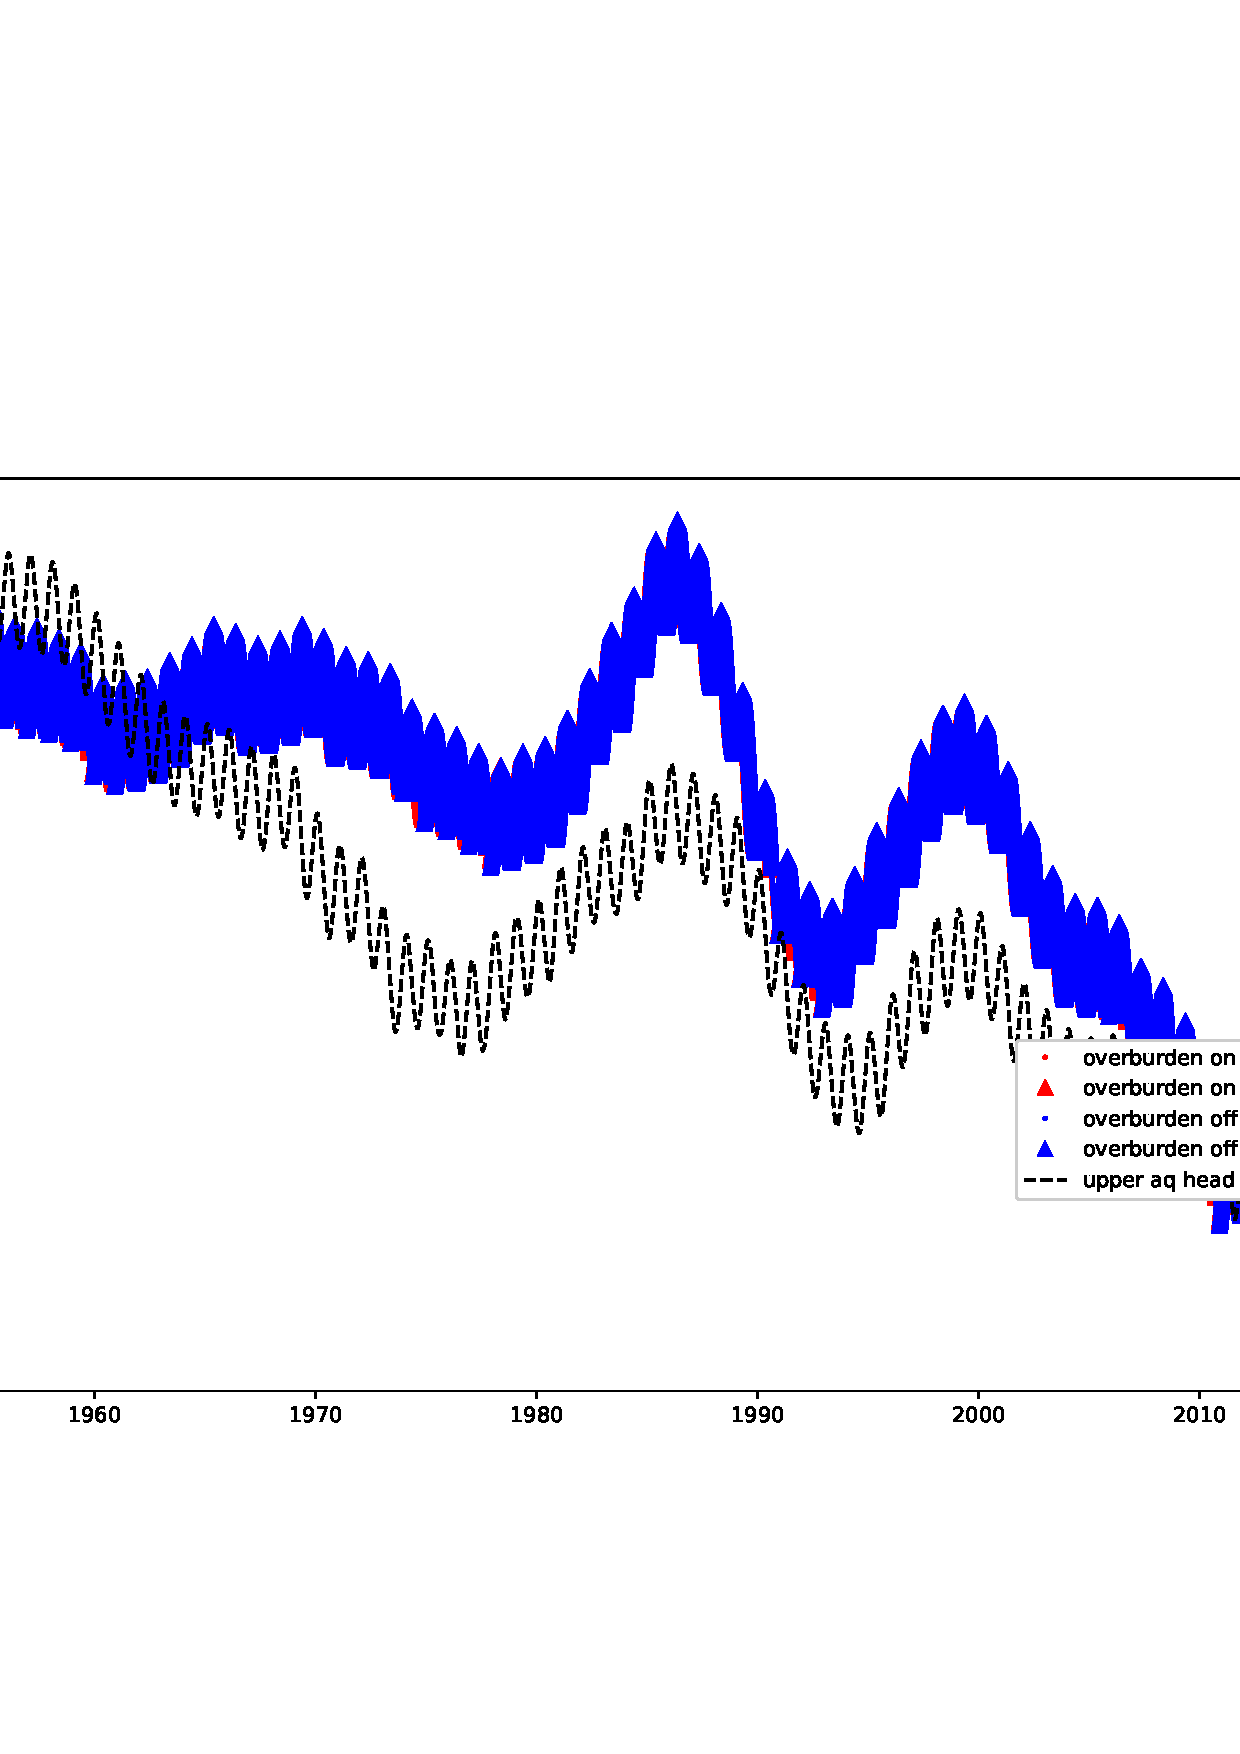
\includegraphics[width=\linewidth]{BasicIllustration.pdf}
\caption{Evolution of head with time at node 21 with and without the impacts of overburden. Red and blue lines are essentially indistinguishable}
\label{fig:overburden1}
\end{figure}

\begin{figure}
\includegraphics[width=\linewidth]{BasicIllustration_ZOOM.pdf}
\caption{Evolution of head with time at node 21 with and without the impacts of overburden. Red and blue lines are now distinguishable as we've zoomed in on a decade}
\label{fig:overburden2}
\end{figure}

\begin{figure}
\includegraphics[width=\linewidth]{BasicIllustration_Timeevolution.pdf}
\caption{Evolution of head with time at node all nodes; 5 timesteps presented. At any given time, the difference (or residual) between the two cases vary with the node. This means that although the overburden stress is applied identically at each node, vertical flow makes the change in head differ spatially.}
\label{fig:overburden3}
\end{figure}

There is a more complex affect which is that the changing overburden stress will alter the timing at which aquifer compaction becomes inelastic. The equations for effective stress (Eq \ref{eqn:effective-stress}) contain both the head and the overburden stress, and hence these two quantities decide whether we use an elastic or inelastic compressibility value (Eq \ref{eq:compressibility-clays}). It seems that this interplay can be somewhat important, and depends on the thickness of the clay lens. In a thin clay lens, the head changes and the overburden changes are approximately in phase, so the overburden stress and head both drop simultaneously. These changes cancel each other out and make it less likely to enter inelastic behaviour than if overburden was not included (Figure \ref{fig:overburden4}). However, for a thick clay lens, head and overburden may no longer be in phase, and in the case that they are substantially out of phase this makes elastic behaviour more common, and hence results in larger head drops (Figure \ref{fig:overburden5}).

\begin{figure}
\includegraphics[width=\linewidth]{BasicIllustration_ElasticInelastic_n5.pdf}
\caption{At node 5, overburden and head are roughly in sync, so including overburden stresses makes only a small difference..}
\label{fig:overburden4}
\end{figure}

\begin{figure}
\includegraphics[width=\linewidth]{BasicIllustration_ElasticInelastic_n21.pdf}
\caption{At node 21, the overburden and head are largely out of sync, which means the overburden stress makes inelastic behaviour less common. Hence, we see a much larger drop in head in the overburden case, as rapid elastic changes are more common. Note the period during the 2000s, when they are in sync again. Here the amplitude of the oscillations in the overburden case is approximately $S_y$ times the oscillations in the upper aquifer head. This reassures me that my code is correctly solving the equations here.}
\label{fig:overburden5}
\end{figure}

\paragraph{Loading efficiency and other details of using overburden in the groundwater flow equation}

The formulation given above assumes that the entirety of the overburden stresses are taken up by the solid matrix, and none by the water itself. In past work, usually focusing on the impact of tidal loading, authors have used a loading efficiency parameter to account for how much stress is carried by the water and the solid matrix. For my purposes, I will note that this is a possibility, but will acknowledge that my model will not account for this. See references: \cite{burgess_terrestrial_2017} and \cite{reeves_incorporation_2000}.


\subsection{Compaction Equations}

When depth is discretised as $(z_0, z_1, ..., z_n)$ and time as $(t_0, t_1, ..., t_m)$, the governing equation for observed surface deformation $s$ is given in Equation \ref{eq:compaction-governing-eqn}.

\begin{equation}
s_k = s(t_k) = s_0 + \sum_{i=0}^{i=k} (s_{i+1} - s_i)
\label{eq:compaction-governing-eqn}
\end{equation}
where $s_0$, the surface deformation at $t_0$, is hereafter set to be zero.

The term $s_{i+1} - s_i$ is equal to the sum across all depths of the product of compressibility $\alpha$ and change in effective stress $\sigma'$:

\begin{equation}
s_{i+1} - s_i = \sum_{j=0}^{n} \alpha(z_j,t_i) [\sigma'(z_j,t_{i+1}) - \sigma'(z_j,t_i) ] \Delta z_j
\label{eq:ds-governing-eqn}
\end{equation}
where compressibility and effective stress are both in general functions of space and time.

Equations \ref{eq:compaction-governing-eqn} and \ref{eq:ds-governing-eqn} can be combined to give the overall governing equation:

\begin{equation}
s(t_k) = \sum_{i=0}^{i=k} \bigg(  \sum_{j=0}^{n} \alpha(z_j,t_i) [\sigma'(z_j,t_{i+1}) - \sigma'(z_j,t_i) ] \Delta z_j \bigg)
\label{eq:compaction-overall-governing-eqn}
\end{equation}

Although Equation \ref{eq:compaction-overall-governing-eqn} is the most general governing equation, for different layers and under different assumptions about variability of compressibility and effective stress, the equation is solved in different forms. A summary of different layers and different solution approaches is given in Table \ref{table:compaction-options}, whilst an explanation of some of the terms are given in the following two sections, `Effective Stress' and `Compressibility'.

\begin{table}[h]
\centering
\begin{tabular}{|c|p{9cm}|} 
\hline
\textbf{Layer type} & \textbf{Soln treatment} \\ 
\hline
Aquifer (connected matrix) & Effective stress as in Equation \ref{eqn:effective-stress} and overburden as in Equation \ref{eq:overburden} if not uppermost layer. Cst head wrt depth, so Equation \ref{eq:compaction-overall-governing-eqn} collapses with n=1. Compressibility constant.\\
\hline 
Aquifer (interbedded clays) & Effective stress as in Equation \ref{eqn:effective-stress} and overburden as in Equation \ref{eq:overburden} even if uppermost layer. Compressibility varies as in Equation \ref{eq:compressibility-clays}.\\
\hline 
Aquitard & Effective stress as in Equation \ref{eqn:effective-stress} and overburden as in Equation \ref{eq:overburden} even if uppermost layer. Compressibility varies as in Equation \ref{eq:compressibility-clays}.\\
\hline 
\end{tabular}
\caption{Summary of compaction equation in different layer types.}
\label{table:compaction-options}
\end{table}


\subsubsection{Effective stress}

Effective stress $\sigma'$ is the difference between overburden stress and pore fluid pressure. Using the relations between pore fluid pressure and hydraulic head in confined and unconfined aquifers respectively, we can write the effective stress term in Equation \ref{eq:compaction-overall-governing-eqn} as follows:

\begin{equation}
\label{eqn:effective-stress} 
\sigma'(z_j,t_{i+1}) - \sigma'(z_j,t_i) =
\begin{cases}
\bigg( \sigma (t_{i+1}) - \sigma(t_i) \bigg) - \rho g \big( h(z_j,t_{i+1}) - h(z_j,t_i) \big) & \text{Confined Aquifer} \\
\bigg( \sigma (t_{i+1}) - \sigma(t_i) \bigg) - \rho g \big( h(z_j,t_{i+1}) - h(z_j,t_i) \big)(1-S_y) & \text{Unconfined Aquifer} \\
\end{cases}
\end{equation}

Note that here, consistent with the groundwater flow equation, the overburden stress $sigma$ is the stress originating above the layer in question. However, we now account for a pressure change due to the changing head in the layer itself; this is only significant in the unconfined aquifer, where it is included as the $(1-S_y)$ term. I neglect the equivalent term for a confined aquifer, which would be $(1-S_s)$, because $S_s << 1$. See \cite{poland_land_1969} for derivations of these. 

Overburden stress varies in general due to any changing mass in layers above the aquifer. We only consider the significant overburden stress of changing saturation in the unconfined aquifer. Mathematically, we can write this as:

\begin{equation}
\label{eq:overburden}
\sigma (t_{i+1}) - \sigma(t_i) = \rho g S_y \big( h^{unconfined}_{i+1} - h^{unconfined}_i \big)
\end{equation}

Note that the code never requires the user to specify which aquifer is confined or unconfined. Instead, it assumes that if the topmost layer is an aquifer, it is unconfined.

\paragraph{Expected effect of including overburden stress}
\label{sec:overburden-compaction}

This section is written prior to coding  up the impact of overburden stress, such that I have an intuition of how the code should respond to the inclusion of overburden stress. 

First, including overburden stresses will alter the groundwater flow equation. For discussion of this, see Section \ref{sec:overburden-gwflow}.

%It will not alter this equation in the unconfined aquifer, since there is no overburden stress above it. However, it will alter things in the confined aquifer. If I assume both aquifers have head levels changing in the same direction, but with the unconfined seeing changes about a third of those in the confined, then a head drop in the confined aquifer will have a corresponding head drop as third as large in the unconfined aquifer. The former drop will encourage water to flow out of confined clays, but the second change will reduce the pressure they experience and therefore somewhat reduce the tendency for water to flow from the clays. Hence, I expect overburden stresses to generally mute the drainage of clays in the confined layers; however, this will be a relatively small impact because the effect will be a third times by $(1-S_y)$, so something like $\frac{2}{9}$ reduction. 

Second, including overburden stresses will alter the compaction equations. This will occur in both the unconfined and confined aquifer, as well as the aquitard. In the unconfined, compaction is simply reduced by a factor of $(1-S_y)$. In the confined and aquitard layers, things are rather more complicated. I use the same logic as before about head in the confined and unconfined showing the same trends but the former having 3x larger magnitude. In this case, a head drop in the confined will, by itself, lead to compaction; however, it will have a smaller head drop in the unconfined to go with it, which will reduce pressure and retard compaction. The size of this effect should be the same as in the above paragraph, so something like a $\frac{2}{9}$ reduction. In the aquitard, we will see similar reductions, although it is harder to think about this and probably not very important. However, there is an additional complexity which arises because the elastic vs inelastic condition is also impacted by the overburden stress. My anticipation is that this won't change too much, but I am not sure. It is hard to get a sense of this. 

%In most applications, overburden stress is assumed constant so Equation \ref{eq:compaction-overall-governing-eqn} is solved with $\sigma'(z_j,t_{i+1}) - \sigma'(z_j,t_i) = \rho g \big( h(z_j,t_{i+1}) - h(z_j,t_i) \big)$.

\subsubsection{Compressibility}

Although in Equation \ref{eq:compaction-overall-governing-eqn}, compressibility varies with time, for most sediment types, it can be considered a constant. The exception to this rule is clays, which can deform both elastically and inelastically depending on the effective stress history they have experienced. This is a complex, non-linear and hysteretic variation, which can nonetheless be written down mathematically and modelled \cite{helm_one-dimensional_1976}. Here, we approximate the behaviour into two classes, elastic and inelastic:

\begin{equation}
\label{eq:compressibility-clays}
\alpha = 
\begin{cases}
\alpha_{ke} & \sigma' < max(\sigma') \\
\alpha_{kv} & \sigma' > max(\sigma') \\
\end{cases}
\end{equation}
Note that $alpha_{kv}$ is much larger (often an order of magnitude) than $alpha_{ke}$. Also note that, when combined with Equations \ref{eqn:effective-stress} and \ref{eq:compaction-overall-governing-eqn}, we often use the skeletal specific storage values rather than compressibilities, since these are related by:

\begin{equation}
\label{eq:skeletal-specific-storage}
\alpha = 
\begin{cases}
S_{ske} = \rho g \alpha_{ke} & \text{Elastic} \\
S_{skv} = \rho g \alpha_{kv} & \text{Inelastic} \\
\end{cases}
\end{equation}

\subsubsection{Comments on solution}

\textbf{Solving at midpoints}

In the case of aquitards and interbedded clays, head and therefore effective stress will vary at every node throughout the clay. In Section \ref{sec:diffusion}, the details of how head is calculated at these nodes are reported. However, in these solutions, the topmost and bottommost nodes are boundary conditions with predetermined head values representing the adjacent interconnected aquifer(s). The head at these nodes does not represent the head in the clay layers, and hence should not be used for compaction calculations. I have `solved' this problem by solving the compaction equation \ref{eq:compaction-overall-governing-eqn} at midpoints between the nodes from the head equation. Hence, the first step in solving the compaction equation in aquitards and interbedded clays is the interpolate (linearly) between nodes in the head equation. This problem does not arise in interconnected coarse layers because these have constant head throughout.

In the aquitards and interbedded clays, Equation \ref{eq:compaction-overall-governing-eqn} is solved as stated in Table \ref{table:compaction-options}, with the proviso as mentioned above that the nodes are the midpoints of the head solution. 

\textbf{How many nodes?}

Experimenting with a 1m thick clay lens led me to believe that you need at least 5 nodes in the groundwater solver equation to get a convergent solution for the compaction equation. If I have time, I will put some images here to that effect.

\section{Input Head Timeseries}

The ultimate objective is that the model will be able to read in head timeseries files in a flexible variety of fileformats. At present, the file format must be two columns of comma-delimited items, of format:

DATE,MEASUREMENT

DATE should be a string of any format and MEASUREMENT should be a number given to any number of significant figures, in the units of metres. We rely on Python's pandas library to automatically read the dates in any format; if this is not working, see the last paragraph of this subsection for a potential manual solution.

Internally, the model uses Python's Datetime module, and dates are stored as numerically as a number of days since 0000-12-31 using the datetime.date2num method. See \url{https://www.w3schools.com/python/python_datetime.asp} and \url{https://matplotlib.org/3.1.1/api/dates_api.html\#matplotlib.dates.date2num}.

There are some potential issues with future head projections beyond the year 2069, as for certain situations Datetime seems to interpret XX69 as 1969 no matter what XX is. If this occurs, you may need to go into the code and manually specify a date format or parser, which is included as a commented out line/lines in the execute model code.

\section{Suggested Hydraulic Parameters}

For convenience, I am keeping a note of suggested hydraulic parameters here. 

\subsection{Specific Storage Values}

This section describes values of Specific Storage $S_s$ which are used in solving the groundwater flow equation (note these will be slightly different to values of skeletal specific storage used for solving the compaction equation). Values are notated in Table \ref{table:Ss-values}.

\begin{table}[h]
\centering
\begin{tabular}{|c|c|p{4cm}|} 
\hline
\textbf{Source} & \textbf{Variable} & \textbf{Value(s)}\\ 
\hline
\cite{faunt_groundwater_2009} & Elastic $S_s$, coarse material, lab and field values & $3.3 \times 10^{-6}$ m$^{-1}$ \\
\hline 
\cite{faunt_groundwater_2009} & Elastic $S_s$, coarse material, values from prev models & $4.6 \times 10^{-6}$ m$^{-1}$\\
\hline
\cite{faunt_groundwater_2009} & Elastic $S_s$, coarse material, value from their model & $3.3 \times 10^{-6}$ m$^{-1}$ \\
\hline
\cite{faunt_groundwater_2009} & Elastic $S_s$, fine material, value from their model & $1.5 \times 10^{-5}$ m$^{-1}$ \\
\hline
\cite{faunt_groundwater_2009} & Elastic $S_s$, fine material, largest value from field/lab studies & $2.5 \times 10^{-5}$ m$^{-1}$ \\
\hline
\cite{faunt_groundwater_2009} & Inelastic $S_s$, fine material, value from their model & $4.6 \times 10^{-4}$ m$^{-1}$ \\
\hline
\cite{faunt_groundwater_2009} & Inelastic $S_s$, fine material, largest value from field/lab studies & $2.2 \times 10^{-3}$ m$^{-1}$ \\
\hline 
\cite{faunt_groundwater_2009} & Inelastic $S_s$, fine material, "previously simulated values" & $9.8 \times 10^{-4}$ m$^{-1}$ \\
\hline 
\cite{smith_modeling_2019} & Inelastic $S_{skv}$, fine material, MAP (median value?) & $1.8 \times 10^{-3}$ m$^{-1}$ \\
\hline
\cite{sneed_hydraulic_2001} & Elastic $S_s$, fine material, mean value from calibrated models & $1.5 \times 10^{-5}$ m$^{-1}$ \\
\hline
\cite{sneed_hydraulic_2001} & Inelastic $S_s$, fine material, mean value from calibrated models & $1.0 \times 10^{-3}$ m$^{-1}$ \\
\hline
\cite{sneed_hydraulic_2001} & Inelastic $S_s$, fine material, value from laboratory testing & Approximately half that of model values \\
\hline
\cite{sneed_hydraulic_2001} & Inelastic $S_s$, Corcoran Clay, value from laboratory testing & In 2 of 3 cases, the C-clay was more compressible (larger Ss) than other clays. \\
\hline
\end{tabular}
\caption{Specific storage values reported in various sources for various lithologies in both elastic and inelastic conditions.}
\label{table:Ss-values}
\end{table}


\section{Validating Results}

\subsection{Existing subsidence data}

Comparing modelled subsidence curves with observational data is one way of confirming the model is behaving reasonably. The TRE Altamira, Envisat and other InSAR datasets are not mentioned here, as I assume that I have documentation on those elsewhere. However, there are a few other datasources which give an indication of whether the model is behaving reasonably.

First, the levelling surveys of the 50s, 60s and 70s can be used to check that the start of the model is behaving sensibly. \cite{poland_land_1975} give data of elevation change of benchmark Y286, near to Hanford, at a third of a foot per year for the 3.6 years prior to 1970. I read these values off Figure 11 using a ruler! 

Second, the California Dept of Transportation and the National Geodetic Survey performed geodetic surveys along Highway 198 in the ''1960s'' and 2004. These data are reported in \cite{sneed_land_2018}; the location is given in Figure 15 and the data in Figure 16. I estimate that my stud site is about halfway between the pentagons at Armona and the ones to the right, so I took an elevation change of 2.5 metres accordingly.

Thirdly, there is a very elusive comment in \cite{swanson_land_1998}, which says: ``Between 1980 and 1993, there was a subsidence differential of up to 2 ft along the canal'', referring to the Homeland Canal which runs a little distance south of Hanford. This datapoint is therefore extemely loose, but gives an idea of the rough amount of subsidence expected in the region in the 80s and early 90s. 

\section{Random notes}

CLAUDIA FAUNT SAID IN A MEETING WITH MEREDITH THAT WHEN THEY STARTED PUMPING CV (1950s???), 30\% OF RECHARGE CAME FROM DRAINAGE OF CLAYS. I have since found this repeated in \cite{sneed_hydraulic_2001} on page 11. Good to know!


\bibliographystyle{plainnat}
\bibliography{Manual3}
\end{document}
